

%\section{Design Method}\label{sec:design_method}
This chapter shows focusses on each of the code generation phases and what our contributions are to this compiler. We describe how we have taken a compiler without support for explicit bypass registers, which is described in Section \ref{sec:basic_compiler_design} and improved, maintained and extended it. 

%Discuss maintaining, process of porting from llvm3.8 to LLVM4.0, and discuss new version LLVM5.0. Mention that this upgrade to 4.0 also drastically improved vectorization because the community develops this constantly. (maybe add example of CNN)

%TODO: move vectorization to here? Noooo.

\section{Back-end Code Generation}\label{sec:code_generation}
We will briefly discuss each of the code generation stages, which includes custom passes and standard passes supplied by the LLVM framework. Before generating code, we use LLVM's front-end to translate a high level language to an intermediate representation, called LLVM-IR. This can be further optimized and used as input for our back-end. We categorize the code generation phases in the back-end in three major categories.

\begin{figure}[H]
\centering
\hspace*{-.12in}
\includegraphics[scale=0.53]{figures/code_generation}
%TODO: change orange to yellow and yellow to orange in picture. 
\caption{Overview of the phases that the back-end is comprised of.}
\label{fig:simd_backend}
\end{figure}
%include an image with the pipeline having all these components.

%TODO: refere to problem where instr have no common operand, so it seems unrelated. 

%TODO: add text that explains the color, instruction selection is copied mostly from another architectures, and was already updated according to our architecture. / Hazard recognizer has partially been copied from other architectures, but was not suitable and has, therefore, been modified and tested. / Delay slot is a custom pass that was already implemented, but we have modified it to be more efficient. / Packetizer pass is as delivered, with a minor modification with hardly any efford.  / Bypass Regs is a custom pass that we developed during the duration of our work.

Firstly, we work on creating a schedule which is depicted in the top row of Figure \ref{fig:simd_backend}. The second row illustrates a collection of phases that do back-end specific transformations. Here we take care of special features that our architecture has. At last, now that we have code for our architecture, namely, an LLVM internal representation of it, we emit assembly or ELF object code (depicted in the rightmost part of the image) that our machine can understand.

%A list of all components that follow in the following section.
\begin{itemize}
	\item \textbf{Instruction Selection:} Uses a DAG, called \texttt{SelectionDAGs}, an abstraction for code representation suitable for phases ranging from Instruction Selection, Legalization to Lowering. Instruction selection is implemented in  \texttt{SimdISelDAGToDAG}, which is derived from \texttt{SelectionDAGISel} and consists of a bunch of transformations to transform specific instructions into instruction that are supported by our architecture. For example, transforming operations on immediate values with a value higher than one byte is partially implemented here. Lowering nodes of the \emph{directed acyclic graph} (DAG) is done in \texttt{SimdISelLowering}, which is derived from \texttt{TargetLowering}. There the SIMD intrinsics and ISD instructions are lowered to \emph{Machine Instructions} (MI) and sequences of MIs.
%\item \textbf{Scheduling:} Transforms a directed acyclic graph into an ordered list of instructions.
%\item \textbf{Register allocation:} Assigns physical registers to virtual registers of a list of instructions in SSA form.
	\item \textbf{Instruction Scheduler:} MIScheduler supplied by LLVM\\
MIScheduler is an instruction scheduler which supports VLIW scheduling. Considering there are two issue slots in this architecture, a VLIW scheduler would meet our requirements very well. One and two schedulers are defined for four-stage pipeline and five-stage pipeline respectively. The four-stage pipeline scheduler is the default one while the five-stage pipeline has the default one and additionally a post register allocation scheduler.
	\item \textbf{Register Allocation:} Greedy Allocator supplied by LLVM\\
	The Greedy allocator is a default allocator in LLVM. Since there is no special requirement to register allocation for now, the default allocator is enough to work. Apart from the default register allocator, there are more register allocators to choose from and it is possible to implement a custom register allocator.
	\item \textbf{Post Register Allocation Scheduler:} A second scheduling pass which we only need if we generate code for five-stage pipeline configuration, otherwise, we disable it. The post RA scheduler uses a schedule hazard recognizer, which decides whether to prefer certain instruction over other instructions. For example, RaW hazards are detected and avoided by this algorithm.
	\item \textbf{Hazard Recognizer:} When the five-stage pipeline is configured, consecutive instructions may have hazards. That is, when an instruction tries to read a register of which the result is not there yet because the operation took two cycles. This pass implements LLVM's \texttt{ScoreboardHazardRecognizer}, which we adapted to detect and resolve these hazards.
	%TODO: check implements / extends / derived
	\item \textbf{Delay Slot Filler:} For this architecture, jumps and branch instructions modify the program counter (PC) during the instruction decode stage. At that point, the instruction that follows the jump has already been fetched. The slot that follows a jump or branch instruction is called a delay slot. This pass aims to utilize delay slots by filling them with useful instructions.% that come after a jump or conditional branch instruction, i.e. instructions that modify the program counter.%VERIFY: `or e.g.?
	\item \textbf{Immediate Extension:} In principle, a one byte immediate value can be specified with an instruction. However, sometimes you may want to use a larger immediate. This pass allows us to use large immediates using \texttt{zimm} and \texttt{simm} instruction. These instructions have a 18 bit operand, that may be used for larger immediates.% will be a prefix of the original 8 bits  or using a shift to put a value in a register (up to 32 bits).
	\item \textbf{Packetizer:} Bundles scalar instructions with vector instructions. For each instruction it consults whether an issue slots is available on which the instruction can execute. This pass implements VLIW packetizer supplied by the LLVM framework.
	\item \textbf{Bypass Registers Allocation:} This pass exploits explicit datapaths by allocating explicit registers in the generated code. This is currently implemented as a post-processing step but can be replaced by any of the approaches discussed in Section \ref{sec:approaches}.
	\item \textbf{Instruction Printer:} MC is a sub-project of LLVM, which uses \texttt{MCInst} as a representation of an instruction, which is different from the code generator's existing notion of an instruction (\texttt{MachineInstr}). It is used during the last code generation stage when printing the instructions to a given output format. We further divide printing for different output formats, including binary format and SIMD assembly language in XAS-format. 
%TODO: move


\end{itemize}
The following sections give a more elaborate discussion on each custom pass and describes their relation to each other.

%TODO: validate and update
\section{Custom Passes}
This section describes the custom passes mentioned in the previous section. Dependencies and relations to other passes are described. After this, the linker, the assembler and the vectorizer are briefly discussed. The disassembler will not be implemented, but is also briefly described in this section.

\begin{table}[t!]
\caption{Relations between architecture design features and code generation phases.}
\begin{center}
\begin{tabular}{@{}l l l@{}}
\toprule
\textbf{Feature} & \textbf{Code Gen. Pass} \\ \hline
Hardware Pipeline 	& Delay Slot Filler 		& The delay slot, which is a product lockstep\\
				&					& pipelining is utilized by this pass.\\
			 	& Hazard Recognizer 	& This pass is necessary for a five-stage \\
				&					& pipeline configuration where not all\\
				&					& instructions have a single cycle latency.\\
Bit-width 			& Immediate Extension 	& With a different bit-width, constants may\\
				&				    	& be lowered in a different way. \\
ISA extension		& Instruction Selection 	& New instructions need to be described in\\
				& \& instruction lowering	& the back-end. \\
Explicit datapaths 	& Bypass Register Allocation & This optional pass is developed to exploit\\
				&					& explicit datapaths. It can be enabled\\
				&					& using compiler flag \texttt{-explicit}. \\
\bottomrule
\end{tabular}
\end{center}
\label{table:rel_feature_pass}
\end{table}%

\subsection{Hazard Recognizer}\label{sec:hazard_recogn}
When generating code for a four-stage pipeline configuration, all instructions have a latency of one cycle. In that case, hazard recognition is not necessary.
In order to support code generation for a five-stage pipeline configuration we have implemented a hazard recognizer. The hazard recognizer is used by the post-RA scheduler to determine if two consecutive instructions can be scheduled after each other. 

\lstset{style=customasm}
\begin{lstlisting}
addi r13, r0, 14
addi r12, r0, 10
mul  r2,  r5, r13  # latency=2
mul  <@\hspace{1px}\textcolor{red!70!black}{r3}\hspace{1px}@>,  r6, r12  # latency=2
add  r2,  r2, <@\hspace{1px}\textcolor{red!70!black}{r3}\hspace{1px}@>   # RaW dependency
\end{lstlisting}

We detect hazards by considering whether an operation has a RaW dependency with instruction that came prior to it. We have a true hazard when the instruction that came prior to it has a latency of more than one. The \emph{post register allocation} (Post-RA) scheduler does a linear scan through the list of operation and queries the hazard recognizer whether an instruction can be scheduled. When it detects a hazard, it will consider other instructions that are ready to be scheduled and if there are none available without hazards, it will insert a no-op.

%It recognizes hazards by looking at whether the current instruction to be scheduled uses a register that is defined by the instruction issued in the previous cycle, which also has a latency of more than one cycle. If this is the case, we have a hazard and the instruction under consideration can not be scheduled in the current cycle. At this point we will consider other instructions that are ready to be scheduled and if there are none available without hazards, we will insert a no-op.
\subsection{Delay Slot Filler}
During the execution of a conditional branch or jump instruction the \emph{program counter} (PC) is modified while the instruction is in the \emph{instruction decode} (ID) stage. A side product of lockstep pipelining which we introduced in Chapter \ref{sec:datapaths}, is that when a jump instruction is being decoded in the ID stage, the next instruction with $PC = PC+4$ has already been fetched from IMEM before the jump is executed. Therefore, the instruction that is followed by the jump instruction is executed presumptuously, which we refer to as a delay slot.

%This slot will be executed before the instruction that the PC points at after modifying the PC and is called delay slot. %TODO: this paragraph can be shorter 

In order assure correct behaviour we intentionally 
%or initially (stood there in the first place)
place a no-op after each jump or branch instruction. However, sometimes we can do better. Namely we can use an instruction from before the jump instruction instead of a no-op. We search backwards to look at the previous two instructions and the instruction that comes after the jump, which are referred to as $prev_1$, $prev_2$ and $next$ respectively. When the backwards search does not fill the delay slot we intentionally insert a no-op, and if there is a vector operation that comes after the delay slot, we also need to insert a vector-nop, so that it will not be bundled with the delay slot later on by the packetizer.

%\captionof{lstlisting}{Fragment of assembly code to illustrate behaviour of the delay slot filler.}\label{lst:delayslot1}
%\begin{center}
%\hspace{2px}\begin{minipage}{.475\textwidth}
%\begin{lstlisting}[frame=tlrb]
%BB0_1:
%    sfne r1, 7
%    add r3, r3, r1
%    bf BB0_1
%    nop
%\end{lstlisting}
%\end{minipage}\hfill
%\begin{minipage}{.475\textwidth}
%\begin{lstlisting}[frame=tlrb]
%BB0_1:
%    sfne r1, 7
%    bf BB0_1
%    add r3, r3, r1
%   <@ @>
%\end{lstlisting}
%%\vspace{1.9em}
%\end{minipage}
%\end{center}

%Possibly scrap this case distinction 
%Add picture from scratch paper showing these cases

\captionof{lstlisting}{Fragment of assembly code to illustrate behaviour of the delay slot filler for case one.}\label{lst:delayslot1}
\begin{center}
\hspace{2px}\begin{minipage}{.475\textwidth}
\begin{lstlisting}[frame=tlrb]
BB0_1:
    v.add r3, r6, r14
    v.add r4, r5, r12
    j BB0_1
    nop
\end{lstlisting}
\end{minipage}\hfill
\begin{minipage}{.475\textwidth}
\begin{lstlisting}[frame=tlrb]
BB0_1:
    v.add r3, r6, r14
    j BB0_1
    nop
    v.add r4, r5, r12
\end{lstlisting}
%\vspace{1.9em}
\end{minipage}
\end{center}

\begin{enumerate}
\item The ideal case is when the previous two instructions are both vector instructions. In that case, the vector instruction prior to the jump instruction can be moved to after it. Now the vector instruction that remains before the jump ($prev_1$) gets bundled with the jump instruction. If there was originally an instruction after to the jump instruction which is not a vector instruction, it would get bundled with the vector instruction that we moved later on. Therefore, we then need to insert a no-op to ensure the delay slot. %the instruction that came after is a scalar instruction, it would be merged with the filled instruction, therefore, in that case we need to add a nop, such that it bundles with the filled vector instruction.
\item When the instruction before the jump ($prev_1$) is a scalar instruction with no dependencies to the jump itself, we can move it to the delay slot. We are now done if we moved a bundled instruction. Otherwise, when there are two vector operations prior to the jump instruction, we can again move one of them to to after the jump, and fully utilize the delay slot.

%\item[3] We also consider the case where $prev_1$ is a vector instruction, and $prev_2$ is not a relational or jump instruction. Since the first case considers both $prev_1$ and $prev_2$ vector instructions, we consider cases where $prev_1$ is a vector and $prev_2$ is scalar operation by this case. %todo: little more in depth explanation of this pass
\end{enumerate}

\captionof{lstlisting}{Fragment of assembly code to illustrate behaviour of the delay slot filler for case two.}\label{lst:delayslot2}
\begin{center}
\hspace{2px}\begin{minipage}{.475\textwidth}
\begin{lstlisting}[frame=tlrb]
BB0_1:
    v.add r3, r6, r14
    v.add r4, r5, r12
    add   r3, r3, r1
    j BB0_1
    nop
\end{lstlisting}
\end{minipage}\hfill
\begin{minipage}{.475\textwidth}
\begin{lstlisting}[frame=tlrb]
BB0_1:
    v.add r3, r6, r14
    j BB0_1
    add   r3, r3, r1
    v.add r4, r5, r12
   <@ @>
\end{lstlisting}
%\vspace{1.9em}
\end{minipage}
\end{center}

%\captionof{lstlisting}{Fragment of assembly code to illustrate behaviour of the delay slot filler for the third case.}\label{lst:delayslot3}
%\begin{center}
%\hspace{2px}\begin{minipage}{.475\textwidth}
%\begin{lstlisting}[frame=tlrb]
%BB0_1:
%    add r3, r3, r1
%    v.add r4, r5, r12
%    j BB0_1
%    nop
%\end{lstlisting}
%\end{minipage}\hfill
%\begin{minipage}{.475\textwidth}
%\begin{lstlisting}[frame=tlrb]
%BB0_1:
%    j BB0_1
%    add r3, r3, r1
%    v.add r4, r5, r12
%   <@ @>
%\end{lstlisting}
%\vspace{1.9em}
%\end{minipage}
%\end{center}
%todo: give case(s) that is not covered, followed by this line
These two cases are illustrated in Listing \ref{lst:delayslot1} and \ref{lst:delayslot2} and were already present but required some modifications during upgrading to LLVM 4.0. We have tried to add a third case because many delay slots were not being utilized, but it had some issues and was removed. Future work may also include to optimize this pass such that more delay slots are utilized.

%TODO: make case distinction here.
%\begin{enumerate}
%	 \item When the two operation before the jump instruction are both vector instructions,  
%\end{enumerate}
%TODO: make pseudo code of 

%Immediate extension 
\subsection{Immediate Extention}\label{sec:immediate_ext}
All immediate operations in Appendix \ref{appendix:i_type_instrs} have as last operand, a one byte immediate. However, sometimes we need larger numbers. Therefore, we lower constants during instruction selection. We distinct three cases:
\begin{enumerate}
\item When the immediate can be expressed with one byte it is trivial. We do not need to change anything.
\item When the immediate value is larger than one byte, but can be expressed with 26 bits, we add a \texttt{zimm} or \texttt{simm} operation in front of it. These operations have a 18 bit immediate that represent the upper 18 bits for the instruction that follows.

\begin{lstlisting}
simm 3          # 3 << 8 = 768
addi r3, r5, 12 # 768 + 12
\end{lstlisting}
\item If the immediate requires more than 26 bits, we add a couple of instructions to put the immediate value in a register. Firstly, the upper 6 bits go to a register and are shifted all the way to the left. Subsequently, the lower 26 bits are added to it, using previous cases.
%TODO: illustrate how the lowering is done.
\begin{lstlisting}
add  r3, r0, 2    # upper 6 bits of the immediate
slli r3, r3, 26   # 2 << 26
zimm 3            # 3 << 8, upper 18 bits
addi r3, r3, 12   # lower 8 bit
\end{lstlisting}
\end{enumerate}

\texttt{ImmExtension} is a class that is derived from \texttt{MachineFunctionPass} and adds a \texttt{zimm} or \texttt{simm} when necessary. Pseudo code for this algorithm can be found in another thesis \cite[Appendix B]{liu_zhenyuan}. 

Our contribution to this is that we extended the range of immediate values from 26 to 32 bits. Furthermore, we resolved a bug that was found in the part that inserts \texttt{simm} instructions for an immediate. We can support even operations with more bits, since carry-using operations can be selected. These operations have three operands: The first two are the normal LHS and RHS, and the third is the input carry flag. The operations can then be chained together for adding and subtracting arbitrarily large values.

\subsection{Packetizer}
Using a packetizer transforms a sequential list of mixed scalar and vector operations into VLIW instructions that contain one scalar and one vector instruction. It does this by using \emph{VLIWPacketizerList} of the LLVM framework. %How do I say this? (of or from or ..) is this the correct way to do it or do you know any better or neater way to do so. 
It searches for packets by going in a top-down approach through the list of operations until the end of the machine function is reached. It aims at filling all operation slots of an instruction, in our case a scalar and a vector operation. If an operation is encountered of a slot which is already full, it ends the packetized instruction and it proceeds to the next packet. 
We show the result of this transformation in Listing \ref{lst:packetizer}. 

\captionof{lstlisting}{Illustration of how a list of mixed scalar and vector operations are transformed into 2-issue instructions.}\label{lst:packetizer}
\begin{center}
\hspace{2px}\begin{minipage}{.45\textwidth}
\begin{lstlisting}[frame=tlrb]
v.addi r2,  r0,  a
add    r11, r10, r0
v.addi r3,  r0,  b
v.lw   r2,  r2,  0
v.lw   r3,  r3,  0
v.addi r11, r11, 4
v.mul  r2,  r3,  r2
v.addi r3,  r0,  c
v.sw   r3,  r2,  0
lw     r10, r11, 0
jr r9
addi   r11, r11, 4
\end{lstlisting}
\end{minipage}\hfill
\begin{minipage}{.5\textwidth}
\begin{lstlisting}[frame=tlrb]
add  r11, r10, r0 || v.addi r2,  r0,  a
                  || v.addi r3,  r0,  b
                  || v.lw   r2,  r2,  0
                  || v.lw   r3,  r3,  0
                  || v.addi r11, r11, 4
                  || v.mul  r2,  r3,  r2
                  || v.addi r3,  r0,  c
lw   r10, r11, 0  || v.sw   r3,  r2,  0
jr r9             || v.nop
addi r11, r11, 4  || v.nop

<@\ @>
\end{lstlisting}
%\vspace{1.9em}
\end{minipage}
\end{center}

%TODO: explain 3.3.

The hazard recognizer described in Section \ref{sec:hazard_recogn} implements a function called \emph{ShouldPreferAnother} which we have implemented to recover from hazards more efficiently. If we have a hazard on the vector slot, you would prefer a vector instruction, because then you immediately resolve that hazard and similarly for the scalar slot. However, this function can also be used to do the opposite, namely, prefer a vector instruction if the previous issued instruction was a scalar instruction and vice versa. Alternating instructions may improve the result of the packetizer. 

\subsection{Bypass Registers Allocation}
This pass exploits explicit registers by allocating them to the generated code. It currently does this as a post-processing step, but it can be moved to anywhere in the compilation chain. We chose to do this as a post-processing step for its simplicity. We need to know at a point in time, which results can be forwarded. Therefore, we model the behaviour of the bypass network at compile-time and use this model to decide whether we can bypass certain operands. We then use liveliness information of variables that we bypass to decide whether we still need to store the result in a register. Effectively, if the variable that we bypassed is dead after a use (denoted by a register \emph{kill}), we do not need to store it anymore because it will not be used later on. 
 % and going through a list of instructions. %We may then use the model to keep the processor pipeline accurate and use it to allocate 
%While the instruction of a basic block are traversed, we use the model of the bypass network to decide whether we can bypass certain operands.

\captionof{lstlisting}{Fragment of assembly code to illustrate operand forwarding and dead result elimination.}\label{lst:explicit_reg_alloc}
\begin{center}
\hspace{2px}\begin{minipage}{.475\textwidth}
\begin{lstlisting}[frame=tlrb]
lw  r1, r10, 1
lw  r2, r10, 2
mul r1, r1,  r2
sw  r1, r10, 0
\end{lstlisting}
\end{minipage}\hfill
\begin{minipage}{.475\textwidth}
\begin{lstlisting}[frame=tlrb]
lw  r1,  r10, 1
lw  --,  r10, 2
mul --,  r1,  LSU
sw  MUL, r10, 0
\end{lstlisting}
%\vspace{1.9em}
\end{minipage}
\end{center}

In the code fragment above we first load two values from memory. Then we multiply them with each other and finally store the result back to memory. The second load produces a result that is immediately used. Therefore, we forward it with operand forwarding as explained in Chapter \ref{sec:datapaths}. We encode this with LSU, because loads are executed by the \emph{load store unit} (LSU). Similarly, the result of the multiplication is immediately used and forwarded using MUL, again, this is the functional unit on which multiplications are executed.

This is a standalone fragment which means that there are no other uses of the variables that we forward. Therefore, the variables are dead after their use and because that use comes from the bypass network and not from a register. According to dead result elimination (introduced in Chapter \ref{sec:datapaths}) we can remove these obsolete stores, which we encode using `$--$'. When an instruction has this as destination operand, the processor will be idle when that instruction is in the writeback stage. 


%Implementation of explicit datapaths using bypass registers.

%TODO: decide: comment or uncomment following section expl bp pass
%\subsection{Explicit Bypass Registers}
%This component implements the pass that we discuss in Section \ref{sec:expl_bp_impl} and thereby, implements the main goal of this project. It allocates explicit bypass registers on a machine function and it does that on a per basic block fashion using information of the pipeline state of other basic blocks. It uses \emph{BypassState} which keeps track of the bypass state of each basic block and can be configured to work on a given input state. This way the state of a pipeline can be analysed and remembered by the \emph{SimdExplicitRegister} pass after execution a basic block.

%\subsection{Instruction Printer}

%END COMPONENT DESCRIPTION

%\subsection{Assembler and Disassembler}

%\subsection{Linker}


%\subsection{Auto-Vectorization}

%is this table usable, can I make it usable?


%Hier komt de uitleg v/d compiler implementatie en design. Bespreek hier eventuele tradeoffs die ik ben tegengekomen en design decisions die ik of anderen gemaakt hebben. Aangezien dit grotendeels een software project is, zou ik hier ook wat aandacht willen besteden aan software details, als in, bachelor software engineering skills erop los laten.  

%\Blindtext

\section{Exploiting Explicit Datapaths}\label{sec:expl_bp_impl}
This section describes the implementation and design decisions of the explicit datapath implementation on the LLVM-based compiler.

\subsection{Design Decisions}\label{sec:design_decisions}
%First, make the design space as large as possible
% tradeoffs/considerations/selection
% 1 or 2 solutions

First, let us list the design decisions. The first design decision is how to encode explicit datapaths such that the hardware knows about bypasses. Then there is the manner of when in the compilation chain does it actually encode these bypasses.
%TODO: extend with other decisions that are added below.

%TODO: add decision of how to encode the bypass registers. Choice to use register index space or add bits to instruction

%TODO: (is explained at class diagram 3.4.3) add decision for predicate flag instructions, we made getStartOperand to skip flagged instructions. Alternatively, it is also possible to ignore any flag operands that are encountered.
\subsubsection{Encoding datapaths}
The first design decision is how to encode that an operand is forwarded. There are two ways to encode that a source operand comes from the bypass network:
\begin{enumerate}[i.]
  \item Add bits to each instruction to specify that a certain operand comes from the bypass network. It requires three bits per source operands because there are five different bypass sources with a five-stage pipeline. Each instruction may have up to two source operands that can be bypassed. Therefore, this approach requires six additional bits to be added to each instruction.
  \item Use register index space to indicate that an operand comes from the bypass network. This requires at most five registers to be reserved because there are at most five bypass sources.
\end{enumerate} 

The approach in which the register index space is used to encode that an operand is bypassed was chosen because the hardware description of the architecture corresponds to that, and because of the nice feature that it does not require any modification to the instruction format.

\begin{figure}[b]
\centering
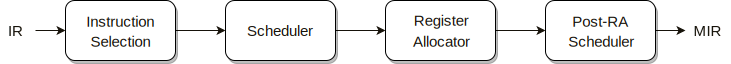
\includegraphics[width=.9\textwidth]{figures/phase_ordering}
\caption{Phase ordering problem.}
\label{fig:phase_ordering}
\end{figure}

\subsubsection{When and how to allocate explicit registers}
Let us start with when to allocate explicit bypass registers. First of all, ideally that would be done before register allocation where there are still virtual registers. The number of virtual registers reduces with each store that is avoided. Thereby, reducing register pressure and relaxing the job for the register allocator.

However, when the register allocator runs out of registers and inserts spill code between two instructions that were already bypassed, this bypass may not be valid anymore and therefore, requiring an additional register to undo that bypass.

Trivially, it is not possible to allocate explicit bypass registers before scheduling, because one needs a schedule to do explicit bypass allocation. %the order of instructions is not known at that time. 
So, alternatively it can be done after register allocation. However, the physical registers that are freed by dead result elimination are not exploited when doing this after RA. Because, if spill code was necessary it has already been inserted when doing this after register allocation. Therefore, it may have redundant spill code and does not gain from reduced register pressure.

To summarize, ideally the explicit datapaths are exploited before register allocation to gain from reduced register pressure. But alternatively, it can be done after register allocation which may potentially have redundant spill code. For the later approach, an effort to clean up redundant spill code may be desired for more efficient code.\\

How to exploit explicit register allocation is a very broad question, in fact this is the main goal of this assignment. Let us split up in two categories of approaches:
\begin{enumerate}[i.]
  \item One way to exploit explicit datapaths is to group instructions close to their use. Moreover, if an instruction is strictly adjacent to its use, it may immediately be bypassed.%Group instructions together and allocate special bypass registers on the fly. Moreover, when this is done before register allocation where we have virtual registers, the number of virtual registers reduces with each bypass that we allocate. Thereby, reducing register pressure and relaxing the job for the register allocator.
  \item Another way to exploit explicit datapaths is by going through a basic block (a code sequence with no branches in except to the entry and no branches out except at the exit) and allocate explicit bypass registers as a post-processing step, in the sense that this is done when the schedule does not change anymore.
\end{enumerate}

The approach in the first category where instructions are grouped together has a problem. In the compilation chain the order in which instructions are executed is first decided by the general scheduler. The register allocator may insert spill code at any place in the schedule. After that, the order may change again by the post-RA scheduler and by the delay slot filler. When a bypass is done early on, it needs to be verified if it is still valid after a change to the schedule has been made.\\

%TODO: now show that grouping instructions is not enough, because this will eventually not cover all mandatory bypasses.

Now let us discuss the second approach that works on a basic block. The assumption in this approach is that the order in which instructions are executed is set and does not change anymore. Therefore, each bypass that is applied stays valid. 
%We can allocate explicit bypass register on an instruction if we have a RaW dependency between that instruction and an instruction in the pipeline state model.
The problem that remains is when there are multiple branches to the basic block. With multiple branches in, the state of the pipeline may be different depending on which branch is taken. This problem is referred to as the join problem which is illustrated by example in Listing \ref{lst:join_problem}. Depending on which branch is taken the value of register \texttt{r7} may be forwarded from \texttt{ALU} when coming from \texttt{\%if}, or from \texttt{MUL} when coming from \texttt{\%else}. Thus, the use of \texttt{r7} in \texttt{\%end} is forwarded from the bypass network, but is non-deterministic and this together with being bypassed is not allowed with explicit datapaths. 

%TODO: add example listing C code left, assembly right that end up in different states, and bypass is not valid!

\captionof{lstlisting}{Fragment of C code with corresponding assembly, to illustrate the join problem.}\label{lst:join_problem}
\begin{center}
\hspace{2px}\begin{minipage}{.475\textwidth}
\lstset{style=customc}
%\begin{lstlisting}[caption=List of instructions.,frame=tlrb]
\begin{lstlisting}[frame=tlrb]
int foo(int a, int b, int c)
{
  if (a > b)
    c += 5;
  else
    c = c * 3;
  c = c - a;
  return c;
}


<@\ @>
\end{lstlisting}
\end{minipage}\hfill
\begin{minipage}{.475\textwidth}
\lstset{style=customasm}
%\begin{lstlisting}[caption=IR-code.,frame=tlrb]
\begin{lstlisting}[frame=tlrb]
$foo:           # a = r5, b = r6 and c = r7
  sfles r5, r6
  bf    $else
  nop
$if:
  add   r7, r7, 5   # r7 in ALU
  j     $end
  nop
$else:
  mul   r7, r7, 3   # r7 in MUL 
$end:
  sub   r3, r7, r5  # r7 from MUL or ALU?
\end{lstlisting}
%\vspace{1.9em}
\end{minipage}
\end{center}

To conclude, the first approach discussed above may improve utilization of the bypass network, but can not be used as a stand-alone approach, since it does not solve the join problem. While the second approach works on a single basic block, it can easily be extended to a larger scope (for example, a function-level scope or a module-level scope). The following sections will show how the join problem can be    tackled when considering a larger scope. 

%When we bypass a value that is defined in another basic block, we require all blocks with a branch to that basic block to have that value in the same bypass source.

%REMOVE TEXT BELOW!!!
%We exploit explicit datapaths by going through a basic block (a code sequence with no branches in except to the entry and no branches out except at the exit) and allocate explicit bypass registers as a post-processing step, in the sense that we do this after scheduling, register allocation, packetizing, etc. Doing this as a post-processing step has advantages compared to doing this early on. 

%TODO: discuss add text below? ask Luc or Roel
%\begin{enumerate}[i.]
%\item When this is done after the packetizer it has bundled `VLIW' instructions consisting of both a scalar and a vector operation which reduces complexity of the bypassing approach.
%\item Another reason to do bypass allocation as a post-processing step is that doing it at an earlier stage, where the code is not certain yet, gives more problems. Each of the custom passes may reorder or insert instructions which may invalidate a bypass already allocated before that point.
%\end{enumerate}
%However, doing it early on also has an advantage.
%TODO: add problem with post-processing approach. Namely, doing this before register allocation reduces register pressure. RA tries to find a physical register for each virtual register. When we change some of these virtual registers with bypass registers already, we end do not need to find a physical register for these, thereby, reducing register pressure.

%clue


%TODO: continue writing xxx 


%This is where I will cover the software details and throw in some UML diagrams.
%\blindtext

\subsection{Join Problem}\label{sec:join_prob}
\begin{figure}[t]
\centering
\subfloat[Fork-join in a loop.]{\includegraphics[width=.345\textwidth]{figures/cfg_fork_join_loop_widend}%
\label{fig:fork_join_loop}}
\hfil
\subfloat[Fork-join in an if-else statement.]{\includegraphics[width=.35\textwidth]{figures/cfg_fork_join_widend}%
\label{fig:fork_join_elif}}
\caption{Fork-join illustration in CFGs.}
\label{fig:fork_join}
\end{figure}

The fork-join model typically branches off (fork) execution at a designated point in the program, and joins (merge) at a subsequent point to resume execution. %In parallel computing, this is a technique often used to spawn multiple processes that execute in parallel, which are at some point joined to sequential execution.
%TODO: if sentence above is added, add illustration of -<==>-
When a value is defined in between the fork and join point and is forwarded to after the join it may be defined in one branch, but not or differently in the other branch or branches. When a bypass is encoded in an instruction, it is statically defined, in the sense that whatever branch is taken the value that is forwarded should always come from the bypass source that is encoded in the instruction. 


\begin{lstlisting}
$A:
   <@$\vdots$@>
$B:
   nop             || v.addi r9,  r0, 32
   nop             || v.lw   r2,  r9, 0
   nop             || v.lw   r3,  r9, 1
   addi <@\hspace{1px}\textcolor{red!70!black}{r3}\hspace{1px}@>, r0, 16 || v.lw   r4,  r9, 2
   ori  r4, r0, 0  || v.addi r10, r0, 64
$C:
   lw   r6, <@\hspace{1px}\textcolor{red!70!black}{r3}\hspace{1px}@>, 3  || v.add  r12, CP, r0
   lw   r6, <@\hspace{1px}\textcolor{red!70!black}{r3}\hspace{1px}@>, 2  || v.add  r13, CP, r0
   lw   r6, <@\hspace{1px}\textcolor{red!70!black}{r3}\hspace{1px}@>, 1  || v.add  r14, CP, r0
$D:
   nop             || v.mul  r12, r4, r12
   nop             || v.mul  r13, r3, r13
   addi r4, r4, 0  || v.add  r9,  CP, r10
   addi r4, r4, 4  || v.add  r12, r12, r13
   sfne r4, 32     || v.mul  r14, r2, r14
   bf $C           || v.add  r14, r14, r12
   addi <@\hspace{1px}\textcolor{red!70!black}{r3}\hspace{1px}@>, <@\hspace{1px}\textcolor{red!70!black}{r3}\hspace{1px}@>, 32 || v.sw   r14, r9, 0
$E:
   <@$\vdots$@>
\end{lstlisting}
%TODO: ask if i need to add loop, or change into loop.

When using the bypass network to forward a value from one basic block to another basic block, it is 



\subsubsection{Resolving Conflicts}\label{sec:conflicts}
When an operand can be bypassed, but has an ambiguous pipeline state, a simple correction is usually sufficient to make it unambiguous such that it can be bypassed. Ambiguous behaviour in the pipeline may occur when bypassing over a join point (a basic block that has multiple predecessors). The bypasses that are allocated when assuming the pipeline state of the most frequently executed predecessor is taken as reference, and when a different bypass would be allocated when assuming the pipeline state of another predecessor block, the other predecessor block is modified such that it matches the bypass allocation given by the reference block. Four cases are considered:

\begin{enumerate}
  \item If the reference forwards a value using \texttt{ALU}, but is not in \texttt{ALU} when another predecessor is executed. Then an operation is inserted to the end of these other predecessors which adds zero to the value that is bypassed.
  \item If the reference forwards a value using \texttt{MUL}, but is not in \texttt{MUL} when another predecessor is executed. Then an operation is inserted to the end of these other predecessors which multiplies the forwarded value with one.
  \item If the reference forwards a value using \texttt{LSU}, but comes from another bypass source by other predecessors. Then the load is copied, and inserted at the end of these other predecessors.
  \item When it is not possible to bypass the value from the reference block, but the other block or blocks do require a value to be bypassed. Then a nop is added to the end of the other predecessor(s) such that the value will be written back before it is used.
\end{enumerate}  

For a five-stage pipeline configuration an additional no-op is added when a multiplication or a load was inserted at the end of a block, so that the result is ready when it is used in the first operation of a basic block. This concludes all cases, however, the \texttt{WB} has not been considered. When the reference block forwards a value from \texttt{WB} over a join point, it requires an instruction to be inserted at a non-trivial position in the basic block, depending on where the uses occur. 


%TODO: add example where both a fix is needed, and a wb.

For this reason, the current implementation does not allow forwarding using \texttt{WB} over a join point. It achieves this by performing a check when the WB source is considered in a block that has multiple predecessors. It checks whether the instruction that defines the value and the instruction that it is forwarded to are in the same basic block, and whether the defining instruction dominates its use. If both conditions hold, then we are still good, since it is just being forwarded within a basic block and not over a join point.

This concludes the implementation of resolving ambiguous pipeline states. The next chapter is devoted to assessing the quality of the generated code by analyzing the simulation results.

%TODO: explain that we take the most-frequently executed predecessor block as reference, and fix all other preds to 'overeenkomen' met die block.

%OTOD: show with contradicting example that this approach doesnt work if also WB is considered. Therefore, it is not possible in the current implementation to bypass from the WB over a joint-point. 

%TODO: add scheduler/before RA/combined scheduling&RA/group instructions together to increase number of bypasses/ etc.
 
 
 
 %TODO: explain the difference between mandatory and non-mendatory bypasses (IN CHAPTER .3.4)

%\subsection{Class Diagrams}\label{sec:explicit_impl}
%%First, make the design space as large as possible
% tradeoffs/considerations/selection
% 1 or 2 solutions

%\begin{figure}[t!]
%\centering
%\includegraphics[width=.9\textwidth]{figures/class_diagram}
%\caption{Class diagram of the implemented approach to support explicit datapaths.}
%\label{fig:class_diagram}
%\end{figure}
